\section{Smoothing}

Function \ccc{CGAL::jet_smooth_point_set} smooths the input point set by projecting each point onto a smooth parametric surface patch (so-called jet surface) fitted over its $k$ nearest neighbors.\\

% % Insert image jet_smoothing.jpg/eps
% \begin{center}
%     \label{Point_set_processing_3-fig-jet_smoothing}
%     % Image
%     \begin{ccTexOnly}
%         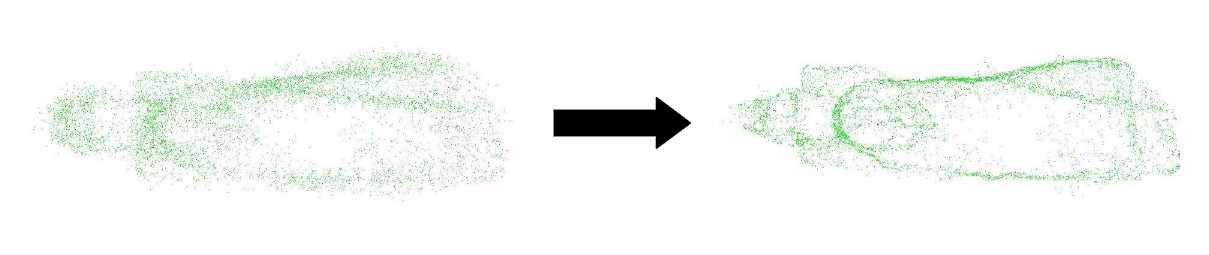
\includegraphics[width=1.0\textwidth]{Point_set_processing_3/jet_smoothing} % omit .eps suffix
%     \end{ccTexOnly}
%     \begin{ccHtmlOnly}
%         <img width="100%" border=0 src="./jet_smoothing.jpg"><P>
%     \end{ccHtmlOnly}
%     % Title
%     \begin{figure}[h]
%         \caption{Point set smoothing}
%     \end{figure}
% \end{center}

\ccExample

The following example generates a set of 9 points close to the $xy$ plane and smooths them using 8 nearest neighbors:
\ccIncludeExampleCode{Point_set_processing_3/jet_smoothing_example.cpp}
